\documentclass{standalone}
\usepackage{tikz}
\usetikzlibrary{patterns, positioning}
\usepackage[sfdefault]{ClearSans} %% option 'sfdefault' activates Clear Sans as the default text font
\usepackage[T1]{fontenc}

\begin{document}
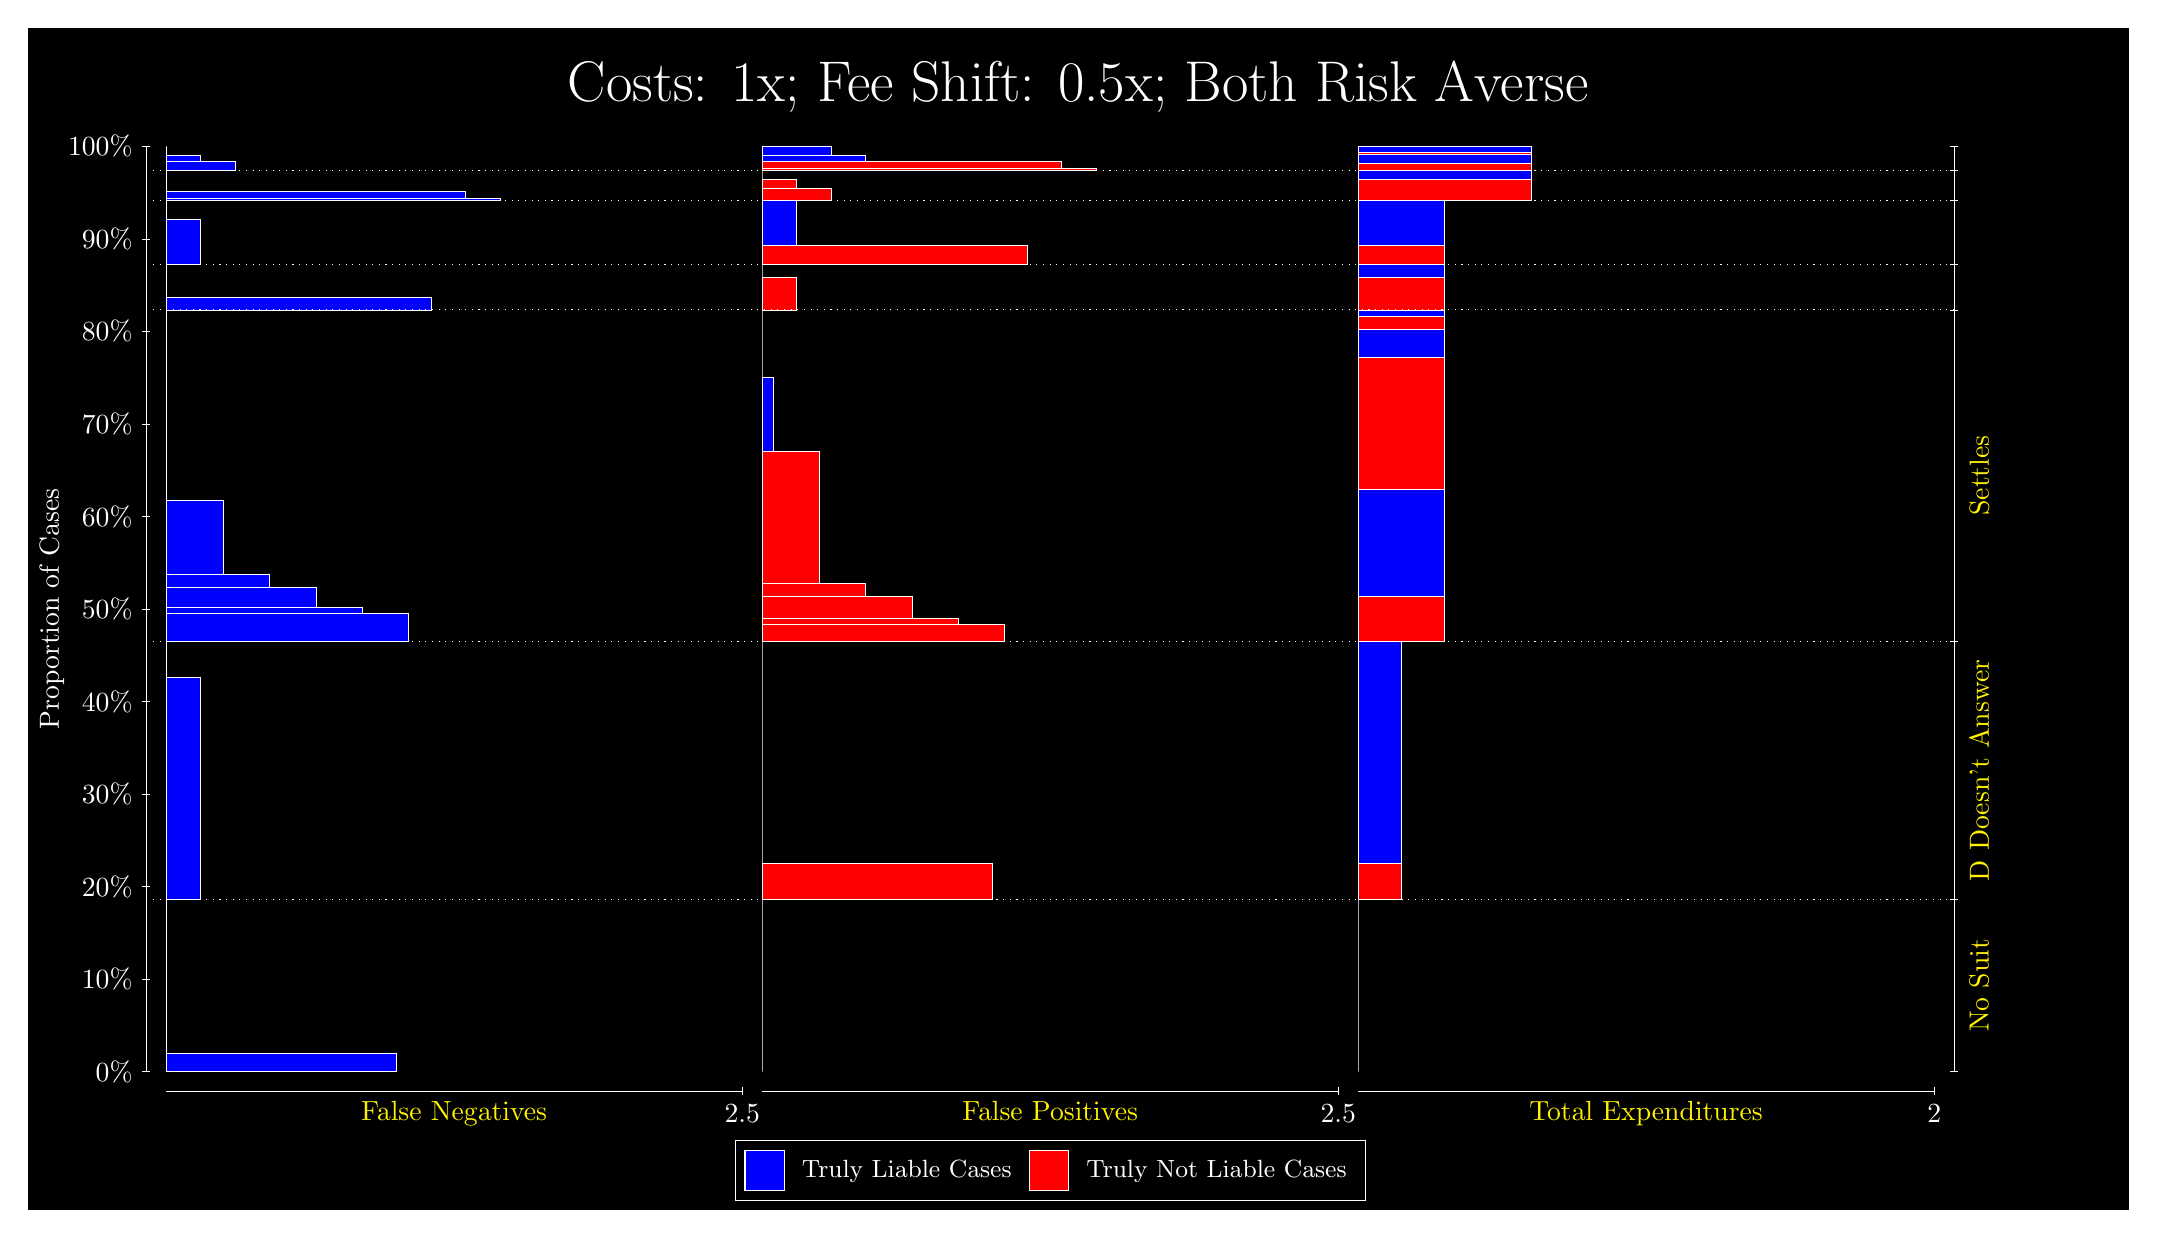
\begin{tikzpicture}
\draw[fill=black] (0,0) rectangle (26.667,15);
\draw[text=white] (0,13.5) rectangle (26.667,15) node[midway] {\huge Costs: 1x; Fee Shift: 0.5x; Both Risk Averse};
\draw[white, very thin] (1.5,1.75) -- (1.5,13.5);
\node[rotate=90, text=white, anchor=center] at (0.3, 7.625) {Proportion of Cases};
\draw[white, very thin] (1.45,1.75) -- (1.55,1.75);
\node[text=white, anchor=east] at (1.45, 1.75) {0\%};
\draw[white, very thin] (1.45,2.925) -- (1.55,2.925);
\node[text=white, anchor=east] at (1.45, 2.925) {10\%};
\draw[white, very thin] (1.45,4.1) -- (1.55,4.1);
\node[text=white, anchor=east] at (1.45, 4.1) {20\%};
\draw[white, very thin] (1.45,5.275) -- (1.55,5.275);
\node[text=white, anchor=east] at (1.45, 5.275) {30\%};
\draw[white, very thin] (1.45,6.45) -- (1.55,6.45);
\node[text=white, anchor=east] at (1.45, 6.45) {40\%};
\draw[white, very thin] (1.45,7.625) -- (1.55,7.625);
\node[text=white, anchor=east] at (1.45, 7.625) {50\%};
\draw[white, very thin] (1.45,8.8) -- (1.55,8.8);
\node[text=white, anchor=east] at (1.45, 8.8) {60\%};
\draw[white, very thin] (1.45,9.975) -- (1.55,9.975);
\node[text=white, anchor=east] at (1.45, 9.975) {70\%};
\draw[white, very thin] (1.45,11.15) -- (1.55,11.15);
\node[text=white, anchor=east] at (1.45, 11.15) {80\%};
\draw[white, very thin] (1.45,12.325) -- (1.55,12.325);
\node[text=white, anchor=east] at (1.45, 12.325) {90\%};
\draw[white, very thin] (1.45,13.5) -- (1.55,13.5);
\node[text=white, anchor=east] at (1.45, 13.5) {100\%};

\draw[white, very thin] (24.457,1.75) -- (24.457,13.5);
\draw[white, very thin] (24.407,1.75) -- (24.507,1.75);
\node[anchor=west] at (24.407, 1.75) {};
\draw[white, very thin] (24.407,3.9363) -- (24.507,3.9363);
\node[anchor=west] at (24.407, 3.9363) {};
\draw[white, very thin] (24.407,7.2133) -- (24.507,7.2133);
\node[anchor=west] at (24.407, 7.2133) {};
\draw[white, very thin] (24.407,11.423) -- (24.507,11.423);
\node[anchor=west] at (24.407, 11.423) {};
\draw[white, very thin] (24.407,12.004) -- (24.507,12.004);
\node[anchor=west] at (24.407, 12.004) {};
\draw[white, very thin] (24.407,12.814) -- (24.507,12.814);
\node[anchor=west] at (24.407, 12.814) {};
\draw[white, very thin] (24.407,13.196) -- (24.507,13.196);
\node[anchor=west] at (24.407, 13.196) {};
\draw[white, very thin] (24.407,13.5) -- (24.507,13.5);
\node[anchor=west] at (24.407, 13.5) {};

\draw[white, very thin, fill=blue] (1.75,1.75) rectangle (4.6775,1.98);
\draw[white, very thin, fill=red] (1.75,1.98) rectangle (1.75,3.9363);
\draw[white, very thin, fill=blue] (1.75,3.9363) rectangle (2.1891,6.754);
\draw[white, very thin, fill=red] (1.75,6.754) rectangle (1.75,7.2133);
\draw[white, very thin, fill=blue] (1.75,7.2133) rectangle (4.8239,7.5699);
\draw[white, very thin, fill=blue] (1.75,7.5699) rectangle (4.2384,7.6495);
\draw[white, very thin, fill=blue] (1.75,7.6495) rectangle (3.6529,7.8978);
\draw[white, very thin, fill=blue] (1.75,7.8978) rectangle (3.0674,8.066);
\draw[white, very thin, fill=blue] (1.75,8.066) rectangle (2.4819,9.0053);
\draw[white, very thin, fill=red] (1.75,9.0053) rectangle (1.75,11.423);
\draw[white, very thin, fill=blue] (1.75,11.423) rectangle (5.1167,11.588);
\draw[white, very thin, fill=red] (1.75,11.588) rectangle (1.75,12.004);
\draw[white, very thin, fill=blue] (1.75,12.004) rectangle (2.1891,12.57);
\draw[white, very thin, fill=red] (1.75,12.57) rectangle (1.75,12.814);
\draw[white, very thin, fill=blue] (1.75,12.814) rectangle (5.9949,12.842);
\draw[white, very thin, fill=blue] (1.75,12.842) rectangle (5.5558,12.927);
\draw[white, very thin, fill=red] (1.75,12.927) rectangle (1.75,13.196);
\draw[white, very thin, fill=blue] (1.75,13.196) rectangle (2.6283,13.313);
\draw[white, very thin, fill=blue] (1.75,13.313) rectangle (2.1891,13.387);
\draw[white, very thin, fill=red] (1.75,13.387) rectangle (1.75,13.5);
\draw[white, very thin, fill=red] (9.3189,1.75) rectangle (9.3189,3.7063);
\draw[white, very thin, fill=blue] (9.3189,3.7063) rectangle (9.3189,3.9363);
\draw[white, very thin, fill=red] (9.3189,3.9363) rectangle (12.246,4.3957);
\draw[white, very thin, fill=blue] (9.3189,4.3957) rectangle (9.3189,7.2133);
\draw[white, very thin, fill=red] (9.3189,7.2133) rectangle (12.393,7.4251);
\draw[white, very thin, fill=red] (9.3189,7.4251) rectangle (11.807,7.5048);
\draw[white, very thin, fill=red] (9.3189,7.5048) rectangle (11.222,7.7844);
\draw[white, very thin, fill=red] (9.3189,7.7844) rectangle (10.636,7.9527);
\draw[white, very thin, fill=red] (9.3189,7.9527) rectangle (10.051,9.6309);
\draw[white, very thin, fill=blue] (9.3189,9.6309) rectangle (9.4652,10.57);
\draw[white, very thin, fill=blue] (9.3189,10.57) rectangle (9.3189,11.423);
\draw[white, very thin, fill=red] (9.3189,11.423) rectangle (9.758,11.839);
\draw[white, very thin, fill=blue] (9.3189,11.839) rectangle (9.3189,12.004);
\draw[white, very thin, fill=red] (9.3189,12.004) rectangle (12.686,12.248);
\draw[white, very thin, fill=blue] (9.3189,12.248) rectangle (9.758,12.814);
\draw[white, very thin, fill=red] (9.3189,12.814) rectangle (10.197,12.965);
\draw[white, very thin, fill=red] (9.3189,12.965) rectangle (9.758,13.083);
\draw[white, very thin, fill=blue] (9.3189,13.083) rectangle (9.3189,13.196);
\draw[white, very thin, fill=red] (9.3189,13.196) rectangle (13.564,13.22);
\draw[white, very thin, fill=red] (9.3189,13.22) rectangle (13.125,13.309);
\draw[white, very thin, fill=blue] (9.3189,13.309) rectangle (10.636,13.383);
\draw[white, very thin, fill=blue] (9.3189,13.383) rectangle (10.197,13.5);
\draw[white, very thin, fill=red] (16.888,1.75) rectangle (16.888,3.7063);
\draw[white, very thin, fill=blue] (16.888,3.7063) rectangle (16.888,3.9363);
\draw[white, very thin, fill=red] (16.888,3.9363) rectangle (17.437,4.3957);
\draw[white, very thin, fill=blue] (16.888,4.3957) rectangle (17.437,7.2133);
\draw[white, very thin, fill=red] (16.888,7.2133) rectangle (17.986,7.7844);
\draw[white, very thin, fill=blue] (16.888,7.7844) rectangle (17.986,9.1402);
\draw[white, very thin, fill=red] (16.888,9.1402) rectangle (17.986,10.818);
\draw[white, very thin, fill=blue] (16.888,10.818) rectangle (17.986,11.175);
\draw[white, very thin, fill=red] (16.888,11.175) rectangle (17.986,11.343);
\draw[white, very thin, fill=blue] (16.888,11.343) rectangle (17.986,11.423);
\draw[white, very thin, fill=red] (16.888,11.423) rectangle (17.986,11.839);
\draw[white, very thin, fill=blue] (16.888,11.839) rectangle (17.986,12.004);
\draw[white, very thin, fill=red] (16.888,12.004) rectangle (17.986,12.248);
\draw[white, very thin, fill=blue] (16.888,12.248) rectangle (17.986,12.814);
\draw[white, very thin, fill=red] (16.888,12.814) rectangle (19.083,13.083);
\draw[white, very thin, fill=blue] (16.888,13.083) rectangle (19.083,13.196);
\draw[white, very thin, fill=red] (16.888,13.196) rectangle (19.083,13.286);
\draw[white, very thin, fill=blue] (16.888,13.286) rectangle (19.083,13.403);
\draw[white, very thin, fill=red] (16.888,13.403) rectangle (19.083,13.426);
\draw[white, very thin, fill=blue] (16.888,13.426) rectangle (19.083,13.5);
\draw[white, dotted] (1.5,3.9363) -- (24.457,3.9363);
\draw[white, dotted] (1.5,7.2133) -- (24.457,7.2133);
\draw[white, dotted] (1.5,11.423) -- (24.457,11.423);
\draw[white, dotted] (1.5,12.004) -- (24.457,12.004);
\draw[white, dotted] (1.5,12.814) -- (24.457,12.814);
\draw[white, dotted] (1.5,13.196) -- (24.457,13.196);
\draw[white, very thin] (1.75,1.5) -- (9.0689,1.5);
\node[text=yellow, anchor=north] at (5.4094, 1.5) {False Negatives};
\draw[white, very thin] (9.0689,1.45) -- (9.0689,1.55);
\node[text=white, anchor=north] at (9.0689, 1.45) {2.5};

\draw[white, very thin] (9.3189,1.5) -- (16.638,1.5);
\node[text=yellow, anchor=north] at (12.978, 1.5) {False Positives};
\draw[white, very thin] (16.638,1.45) -- (16.638,1.55);
\node[text=white, anchor=north] at (16.638, 1.45) {2.5};

\draw[white, very thin] (16.888,1.5) -- (24.207,1.5);
\node[text=yellow, anchor=north] at (20.547, 1.5) {Total Expenditures};
\draw[white, very thin] (24.207,1.45) -- (24.207,1.55);
\node[text=white, anchor=north] at (24.207, 1.45) {2};

\node[text=yellow, centered, rotate=90] at (24.777, 2.8432) {No Suit};
\node[text=yellow, centered, rotate=90] at (24.777, 5.5748) {D Doesn't Answer};
\node[text=yellow, centered, rotate=90] at (24.777, 9.3181) {Settles};





\draw (12.978300999999998,1.5) node[draw=none] (baseCoordinate) {};
\begin{scope}[align=center]
        \matrix[scale=0.5, draw=white, below=0.5cm of baseCoordinate, nodes={draw}, column sep=0.1cm]{
            \node[rectangle, draw, minimum width=0.5cm, minimum height=0.5cm, fill=blue] {}; &
            \node[draw=none, font=\small, text=white] (B) {Truly Liable Cases}; &
            \node[rectangle, draw, minimum width=0.5cm, minimum height=0.5cm, fill=red] {}; &
            \node[draw=none, font=\small, text=white] (B) {Truly Not Liable Cases}; \\
            };
\end{scope}

\end{tikzpicture}
\end{document}